\section{Database}
In this section we will present the design of our database.
Our design will support the concepts that we have introduced, namely project groups and project group members discussed in~\secref{sec:projectgroup}.

Recall that we are designing to comply with a relational database, more specifically an SQL databse as described in~\secref{sub:constraints}.

\subsection{Project Group}
A project group consists of different elements.
How these elements are represented in the database is presented here.
One core elements is the 

A project group must be identifiable by both human and computers.
To make a project group identifiable by humans we give them a short name that must be unique among other project groups.
The field that holds the short name in the project group relation is called \vari{shortname}.
Initially it may seem that the short name could be used general identifier (both for humans and computers) since a short name is unique.
However, this name might be changed during the lifespan of a project group.
We would much rather prefer an identifier that is constant for a project group, to a avoid race conditions.
An example of a race condition in this system could be a user trying to access a project group with an identifier (the short name in this case) while another user is changing the short name of the group.
Should the short name be changed before the first user is trying to access the project group, the request will fail because the identifier that he is holding is deprecated.

We choose to have a numeric auto-incrementing \vari{id} field to identify the project groups.
This cannot be set or changed by the users of the system.
%Ultimately a databse administrator could change it directly in the database, but we cannot guard gainst this assuming the database administrator has super user privelges.

One could argue that the numeric id field could be used as human identifier as well.
However, it is much easier for a humans to remember and associate an alphanumeric name than an arbitrary number.
In summary a project group has two identifiers; the numeric \vari{id} and the alpha numeric \vari{shortname}.

We decided to give the project group the following attributes. 
\begin{itemize}
	\item An id to identify the group. 
	\item A short name to easily identify the group for humans. 
	\item The full name of the group. 
	\item A timestamp for its creation. 
	\item A set of members. 
\end{itemize}

\subsubsection{Project Group Members}
The set of members denotes a relation between project groups and users and we give it the following attributes: 
\begin{itemize}
	\item An id, which is Moodle convention. \cite{moodledb}.
	\item A reference to the related project group.
	\item A reference to the related user.
	\item A role denoting the type of membership the user has to the group.
	\item A timestamp for its creation.
	\item A timestamp for the last update to the membership. 
\end{itemize}
The database scheme can be seen in~\figref{fig:projectgroupsdb}. 
The user entity is an inbuilt part of Moodle and is not modeled by us. 
\begin{figure}
	\centering
		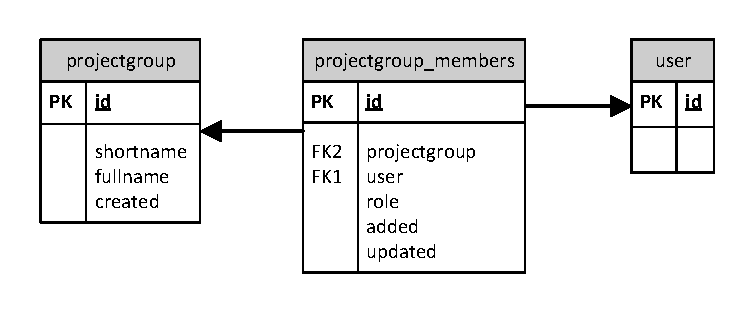
\includegraphics{images/projectgroupsdb.pdf}
	\morscaption{The database scheme of project groups and memberships. The data fields of the user table is omitted for brevity}
	\label{fig:projectgroupsdb}
\end{figure}

%To test the scheme for redundancy we check to see that the scheme conforms to boyce-codd normal form (BCNF). To check this we 

